\documentclass[a4paper]{ltxdoc}

\usepackage[UTF8]{ctex}
\usepackage{unicode-math}
\usepackage{caption}
\usepackage{booktabs}
\usepackage{xcolor}
\usepackage{listings}
\usepackage[perpage]{footmisc}
\usepackage{hypdoc}
\usepackage{amsfonts}
\usepackage{amsmath}
\usepackage{float}
\usepackage{graphicx}

\usepackage{geometry}
\geometry{left=3.3cm, right=3.3cm, top=2.5cm, bottom=3.0cm}

\usepackage{color}

\makeatletter

% 设置字体
\IfFileExists{/System/Library/Fonts/Times.ttc}{
  \setmainfont{Times}
  \setsansfont[Scale=MatchLowercase]{Helvetica}
  \setmonofont[Scale=MatchLowercase]{Menlo}
  \xeCJKsetwidth{‘’“”}{1em}
}{}
\unimathsetup{
  math-style=ISO,
  bold-style=ISO,
}
\IfFontExistsTF{xits-math.otf}{
  \setmathfont[
    Extension    = .otf,
    BoldFont     = *bold,
    StylisticSet = 8,
  ]{xits-math}
  \setmathfont[range={cal,bfcal},StylisticSet=1]{xits-math.otf}
}{
  \setmathfont[
    Extension    = .otf,
    BoldFont     = XITSMath-Bold,
    StylisticSet = 8,
  ]{XITSMath-Regular}
  \setmathfont[range={cal,bfcal},StylisticSet=1]{XITSMath-Regular.otf}
}

% 定义一些命令用于写文档
\newcommand\TeXLive{\TeX{} Live}
\newcommand\unicodechar[1]{U+#1(\symbol{"#1})}
\DeclareRobustCommand\file{\nolinkurl}
\DeclareRobustCommand\env{\texttt}
\DeclareRobustCommand\pkg{\textsf}
\DeclareRobustCommand\cls{\textsf}
\DeclareRobustCommand\opt{\texttt}

% 在 doc 的基础上增加 option 的描述
\def\DescribeOption{\leavevmode\@bsphack\begingroup\MakePrivateLetters
  \Describe@Option}
\def\Describe@Option#1{\endgroup
              \marginpar{\raggedleft\PrintDescribeOption{#1}}%
              \SpecialEnvIndex{#1}\@esphack\ignorespaces}
\@ifundefined{PrintDescribeOption}
   {\def\PrintDescribeOption#1{\strut \MacroFont #1\ }}{}

% 调整列表的格式
\setlength\partopsep{\z@}
\def\@listi{\leftmargin\leftmargini
            \parsep \z@
            \topsep \z@
            \itemsep \z@}
\let\@listI\@listi
\@listi

% listings 的样式
\lstdefinestyle{lstshell}{
  basicstyle      = \small\ttfamily,
  backgroundcolor = \color{lightgray},
  language        = bash,
}
\newcommand\shellcmd[1]{\colorbox{lightgray}{\lstinline[style=lstshell]|#1|}}
\lstnewenvironment{shell}{\lstset{style=lstshell, gobble=2}}{}
\lstnewenvironment{latex}{%
  \lstset{
    basicstyle = \small\ttfamily,
    frame      = single,
    gobble     = 2,
    language   = [LaTeX]TeX,
  }%
}{}

\hypersetup{
  allcolors         = blue,
  bookmarksnumbered = true,
  bookmarksopen     = true,
}
\makeatother


\begin{document}



\title{DGP-Homework7}
\author{高悟恒 }
\date{\qquad 2020-11-14}
\maketitle



一.问题描述:\\
对三角网格进行简化。

二.算法:\\
1.QEM:\\
对每个顶点i及其所有相邻的三角面j,计算顶点的Q(Quadratic error Matrix):
\begin{equation}
Q_i=\sum_{j\in N(i)}\bar{n_j}\bar{n_j}^T,\bar{n_j}=(n_j,-d_j),d_j=n_j^Tx_i
\end{equation}
其中$n_j$为三角面j的法向。\\
之后可以据此计算每条边的$Q^e$为两个顶点的$Q^v$的和。对于每条边可以计算一个目标顶点位置$\bar{v}$:
\begin{equation}
\begin{pmatrix}q_{11}&q_{12}&q_{13}&q_{14}\\q_{12}&q_{22}&q_{23}&q_{24}\\q_{13}&q_{23}&q_{33}&q_{34}\\0&0&0&1\end{pmatrix}\bar{v}=\begin{pmatrix}0\\0\\0\\1\end{pmatrix}
\end{equation}
注意到上式左边矩阵可能奇异,此时选取$\bar{v}=(v_0+v_1)/2$。\\
因此对每条边可以定义代价为:
\begin{equation}
cost=\bar{v}^TQ^e\bar{v}
\end{equation}
每次选取代价最小的边移除,并且更新所有与顶点相邻边的代价。




三.实验结果:

\begin{figure}[H]
  \centering
 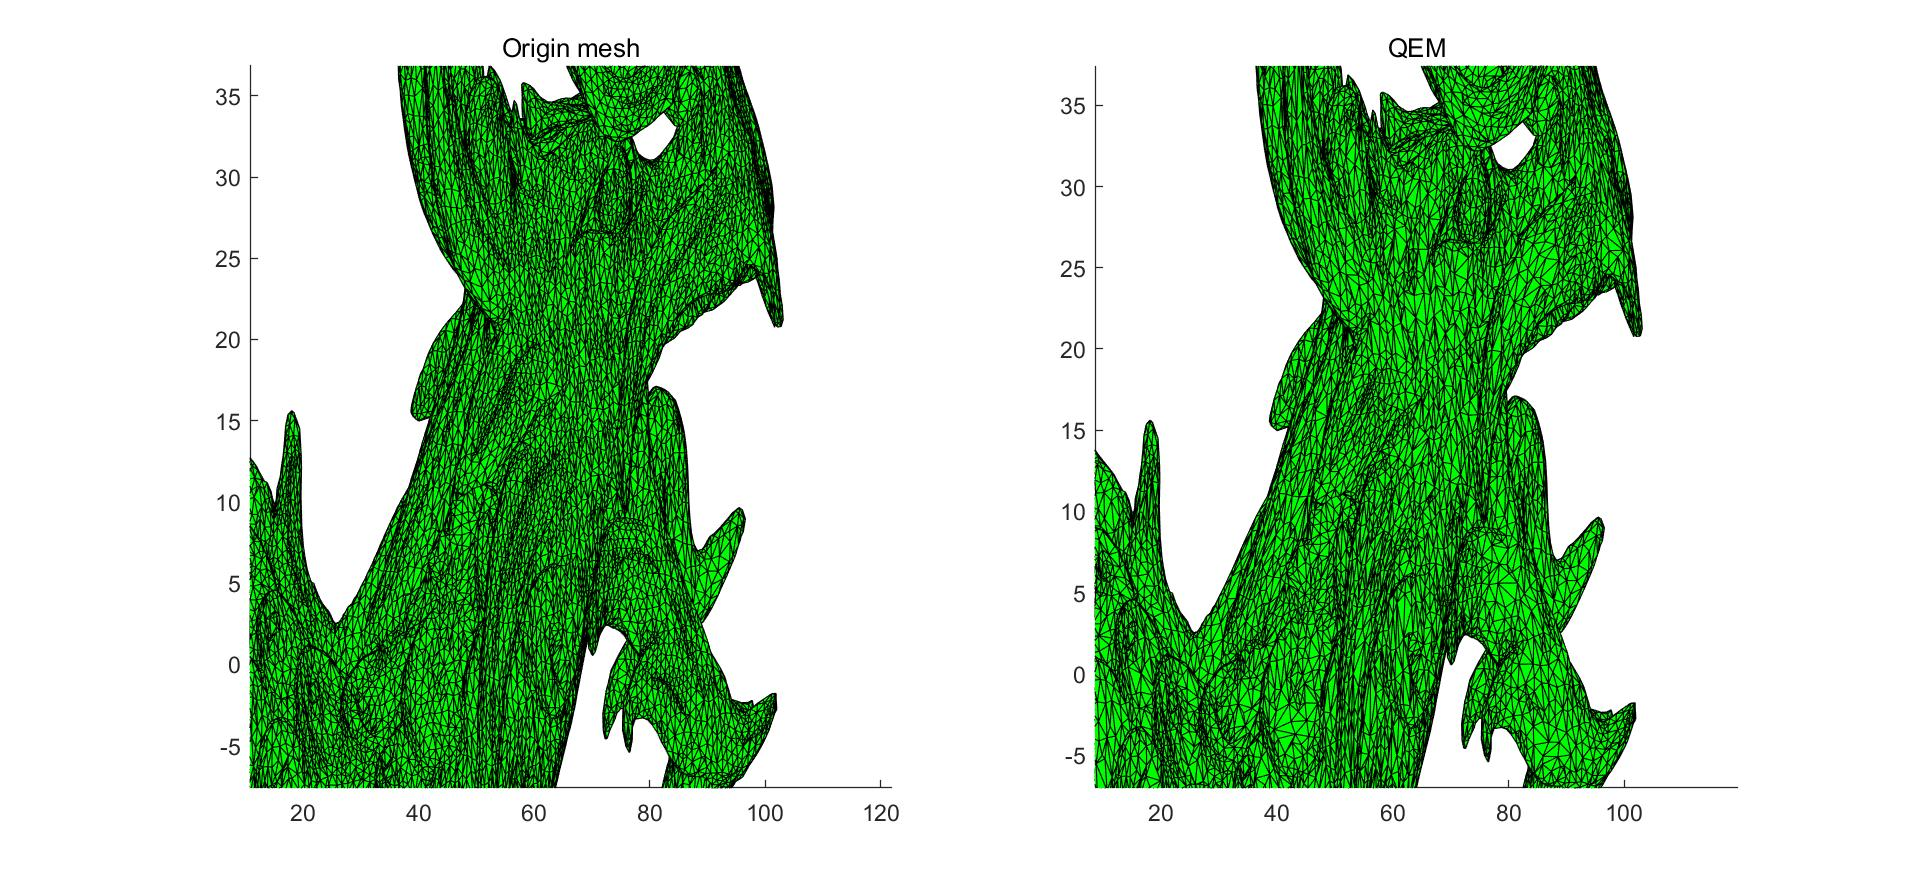
\includegraphics[width=1.0\textwidth]{fig1.jpg}
  \caption{原始龙网格及去掉四分之一顶点的网格}
\end{figure}
\begin{figure}[H]
  \centering
 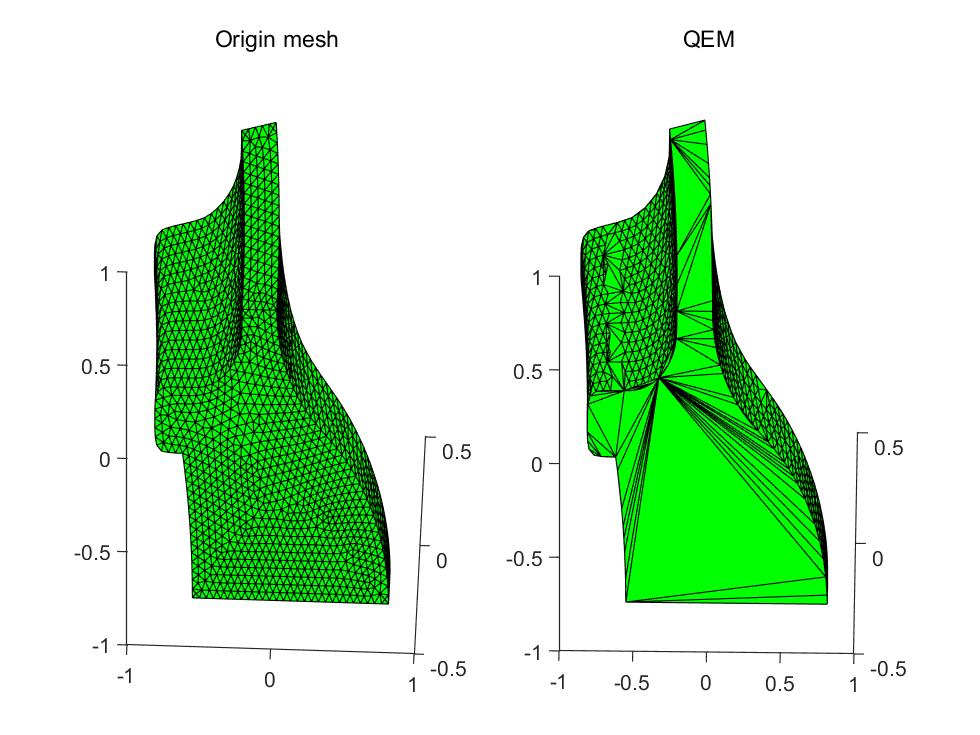
\includegraphics[width=1.0\textwidth]{fig2.jpg}
  \caption{风扇底盘及简化到一半顶点的风扇底盘}
\end{figure}













\end{document}
